\documentclass{article}
\usepackage[utf8]{inputenc}

\title{CCG Simulation}
\author{Piotr Jasik, Damian Zimon}

\usepackage{natbib}
\usepackage{graphicx}
\usepackage{pbox}
\usepackage{float}
\usepackage{xcolor}
\usepackage{caption}
\usepackage{tikz}
    \usetikzlibrary{
        arrows,
        shadows,
        shapes
    }
\usepackage{pgfplots}
\begin{document}

\maketitle

\section{Rules of the game}
    The main objective of the game is to achieve the highest possible Strength score. 
    Player begin the game by drawing \textcolor{red}{5} cards from their deck.
    At the beginning of a turn, players draw a card from their deck.
    Players take turns playing one card each.
    Played card adds it's Strength value to the corresponding player's score. 
    In addition, cards interact with each other e.g. by boosting Attributes or by manipulating Strength score. 
    The game has 2 end conditions: 
    
    \begin{enumerate}
        \item After \textcolor{red}{10} turns.
        \item Player accumulates a lead of \textcolor{red}{50} points over the other player.
    \end{enumerate}
    
    The player with the higher score is considered a winner.

\section{Rules of deck creation}
    
    Each player starts the game with his own deck of \textcolor{red}{30} cards. 
    The card can be chosen from a pool of \textcolor{red}{100} cards.

\section{Rules of pool generation}
    
    The pool, from which the decks will be created, consist of \textcolor{red}{100} cards, 
    that have randomly generated properties.

\subsection{Power Level of a card}
    
    Cards begin with randomly generated card Power Level value.  Whenever a property 
    is assigned to a card, it is then substracted from the card Power Level value. 
    This value can never be negative. The balance of the game, which can be set before 
    the beginning of the game to any value between 0 and 5, determines the upper and lower bound from which the Power Level value is generated:
    
    \begin{center}
        $Power Level = 25\pm \textcolor{red}{Balance}$
    \end{center}
    
\subsection{Card Properties}

\subsubsection{Card Strength}

    First attribute of each card is it's Strength. It's the main factor in calculating Strength score. Other propeties may further manipulate it's value - usually by decreasing your opponent's card's Strength, while increasing your own. Strength value is randomly generated, assuming values shown below.

\begin{center}
   $1 \leq Strength \leq 10$   
\end{center}
  
\subsubsection{Card Attributes}

    $1 \leq Attribute \leq 5$
\subsubsection{Card Traits}
    The last property of a card are Traits. It's a predefined list of additional effects that impact the course of the game. Each Trait has a Power Level cost, which corresponds to how much of Power Level is decreased from a card in the process of card generation.
\begin{table}[h]
    \begin{tabular}{ | c | c | l | c |}
        \hline
        Cost & Name & Effect & Symbol\\ \hline
        12 & Swift & Play another card this round. & $>>$ \\  \hline
        8 & Symbiotic & Double the Strength of your next card with this trait. & * \\ \hline
        4 & Poisonous &\pbox{25cm}{If you control 3 cards with this trait, 
        \\destroy random card played by your opponent.}  & $\dagger$ \\  \hline
        3 & Empowering & Your next card's attributes are increased by 1 each. & +\\ \hline
        2 & Sabotaging & Your opponent's next card loses random attribute (set it to 0.) & $\downarrow$ \\ \hline
        1 & Supporting & Your next card Strength is increased by 1.& $\uparrow$ \\ \hline
    \end{tabular}
\caption{List of traits}
\label{tab:traitcost}
\end{table}

\clearpage

\subsection{Example of a single card generation}
\centering
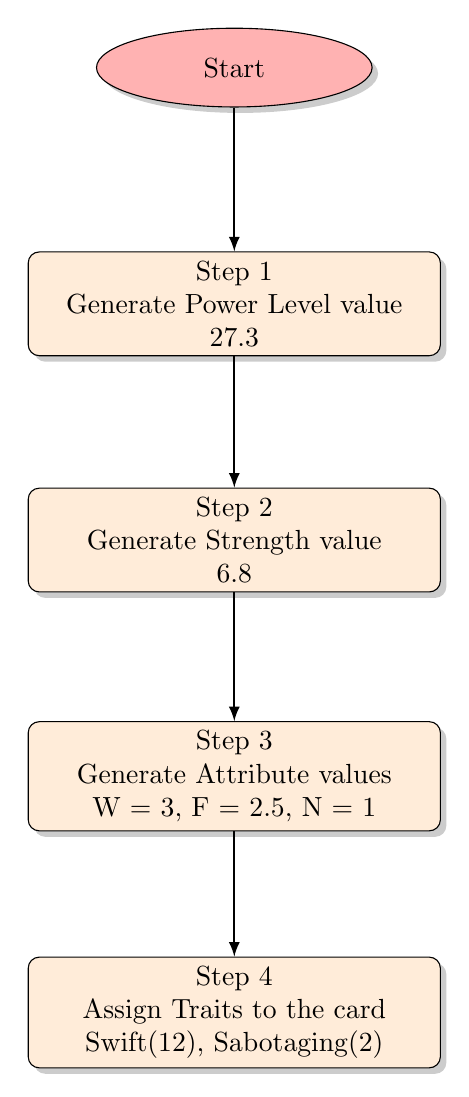
\begin{tikzpicture}[
baseshape/.style={minimum width=3.5cm, minimum height=1cm,text centered, font=\normalsize,draw=black, drop shadow=black!40},
startstop/.style={baseshape, ellipse, fill=red!30},
io/.style={baseshape, trapezium, trapezium stretches=true, 
trapezium left angle=70, trapezium right angle=110, fill=blue!30},
process/.style={baseshape, rectangle, rounded corners, text width=5cm, fill=orange!15},
decision/.style={baseshape, diamond, minimum width=1cm, fill=green!30},
arrow/.style={thick, -latex}, node distance=3cm,
]

\node (step0) [startstop] {Start}; 
\node (step1) [process, below of=step0] {Step 1 \\ Generate Power Level value \\ 27.3};
\node (step2) [process, below of=step1] {Step 2 \\ Generate Strength value \\ 6.8};
\node (step3) [process, below of=step2] {Step 3 \\ Generate Attribute values \\ W = 3, F = 2.5, N = 1};
\node (step4) [process, below of=step3] {Step 4 \\ Assign Traits to the card\\ Swift(12), Sabotaging(2)};

\draw[arrow] (step0) -- (step1);
\draw[arrow] (step1) -- (step2);
\draw[arrow] (step2) -- (step3);
\draw[arrow] (step3) -- (step4);

\end{tikzpicture}
\end{document}